\documentclass[unicode,11pt,a4paper,oneside,numbers=endperiod,openany]{scrartcl}

\usepackage{ifthen}
\usepackage[utf8]{inputenc}
\usepackage{graphics}
\usepackage{graphicx}
\usepackage{hyperref}

\pagestyle{plain}
\voffset -5mm
\oddsidemargin  0mm
\evensidemargin -11mm
\marginparwidth 2cm
\marginparsep 0pt
\topmargin 0mm
\headheight 0pt
\headsep 0pt
\topskip 0pt        
\textheight 255mm
\textwidth 165mm

\newcommand{\duedate} {}
\newcommand{\setduedate}[1]{%
\renewcommand\duedate {See iCorsi for due date}}
\newcommand\isassignment {false}
\newcommand{\setassignment}{\renewcommand\isassignment {true}}
\newcommand{\ifassignment}[1]{\ifthenelse{\boolean{\isassignment}}{#1}{}}
\newcommand{\ifnotassignment}[1]{\ifthenelse{\boolean{\isassignment}}{}{#1}}

\newcommand{\assignmentpolicy}{
\begin{table}[h]
\begin{center}
\scalebox{0.8} {%
\begin{tabular}{|p{0.02cm}p{16cm}|}
\hline
&\\
\multicolumn{2}{|c|}{\Large\textbf{HPC Lab ---  Submission Instructions}}\\
\multicolumn{2}{|c|}{\large\textbf{(Please, notice that following instructions are mandatory: }}\\
\multicolumn{2}{|c|}{\large\textbf{submissions that don't comply with, won't be considered)}}\\
&\\
\textbullet & Assignments must be submitted to \href{https://www.icorsi.ch}{iCorsi} (i.e. in electronic format).\\
\textbullet & Provide source files (e.g. C/C++ files, Matlab). 
If you are using libraries, please add them in the file. Sources must be organized in directories called:\\
\multicolumn{2}{|c|}{\textit{Project\_number\_lastname\_firstname}}\\
& and  the  file must be called:\\
\multicolumn{2}{|c|}{\textit{project\_number\_lastname\_firstname.zip}}\\
\multicolumn{2}{|c|}{\textit{project\_number\_lastname\_firstname.pdf}}\\
\textbullet &  The TAs will grade your project by reviewing your project write-up, and looking at the implementation 
                 you attempted, and benchmarking your code's performance.\\

\textbullet & You are allowed to discuss all questions with anyone you like; however: (i) your submission must list anyone you discussed problems with and (ii) you must write up your submission independently.\\
\hline
\end{tabular}
}
\end{center}
\end{table}
}
\newcommand{\punkte}[1]{\hspace{1ex}\emph{\mdseries\hfill(#1~\ifcase#1{Points}\or{Points}\else{Points}\fi)}}


\newcommand\serieheader[6]{
\thispagestyle{empty}%
\begin{flushleft}

\includegraphics[width=0.4\textwidth]{usi_inf.png}
\end{flushleft}
  \noindent%
  {\large\ignorespaces{\textbf{#1}}\hspace{\fill}\ignorespaces{ \textbf{#2}}}\\ \\%
  {\large\ignorespaces #3 \hspace{\fill}\ignorespaces #4}\\
  \noindent%
  \bigskip
  \hrule\par\bigskip\noindent%
  \bigskip {\ignorespaces {\Large{\textbf{#5}}}
  \hspace{\fill}\ignorespaces \large \ifthenelse{\boolean{\isassignment}}{\duedate}{#6}}
  \hrule\par\bigskip\noindent%  \linebreak
 }

\makeatletter
\def\enumerateMod{\ifnum \@enumdepth >3 \@toodeep\else
      \advance\@enumdepth \@ne
      \edef\@enumctr{enum\romannumeral\the\@enumdepth}\list
      {\csname label\@enumctr\endcsname}{\usecounter
        {\@enumctr}%%%? the following differs from "enumerate"
	\topsep0pt%
	\partopsep0pt%
	\itemsep0pt%
	\def\makelabel##1{\hss\llap{##1}}}\fi}
\let\endenumerateMod =\endlist
\makeatother




\usepackage{textcomp}





\usepackage{listings}
\usepackage{hyperref}
\usepackage{subcaption}
\usepackage{multirow}



\begin{document}


\setassignment

\serieheader{High-Performance Computing Lab}{Institute of Computing}{Student: Paolo Deidda}{Discussed with: FULL NAME}{Solution for Project 1}{}
\newline

% \assignmentpolicy
% In this project you will practice memory access optimization, performance-oriented programming, and OpenMP parallelizaton 
% on the Rosa Cluster .  

\tableofcontents
\newpage

\section{Rosa Warm-Up \punkte{5}}
\subsection{exercise 1}
The \textbf{module system} is a utility that allows the user to dynamically manage their software environment on the Rosa HPC cluster and to load different compilers, libraries and applications in order to modify environment variagles (like PATH, LD LIBRARY PATH, MANPATH, etc.) without creating conflicts between different software versions or dependencies.    

As riported in the USI resource page the module system provides several commands to manage the environment.

\begin{itemize}
    \item \texttt{module avail} -- lists all available modules (on the current system)
    \item \texttt{module list} -- lists all currently loaded modules
    \item \texttt{module show} -- display information about
    \item \texttt{module load} -- loads module
    \item \texttt{module switch} -- unloads, loads
    \item \texttt{module rm} -- unloads module
    \item \texttt{module purge} -- unloads all loaded modules
\end{itemize}

\subsection{exercise 2}
The \textbf{Slurm} (Simple Linux Utility for Resource Management) is a job scheduler for Linux clusters.
Main features of Slurm are:
\begin{itemize}
    \item Job scheduling and resource management
    \item Framework for starting, executing, and monitoring work (jobs) on a set of allocated nodes
    \item Queuing management to handle multiple users and jobs
\end{itemize}

The two main components are:
\begin{itemize}
    \item \textit{sulurmd}: the deamnon that runs on each compute node responsible for launching, monitoring, and terminating jobs
    \item \textit{slurmctld}: the central management daemon that manages job queues and allocates resources
\end{itemize}

Main commands:
\begin{itemize}
    \item \texttt{srun}: submit a job for execution
    \item \texttt{sbatch}: submit a batch job
    \item \texttt{squeue}: view the status of jobs in the queue
    \item \texttt{scancel}: cancel a job
    \item \texttt{salloc}: allocate resources for an interactive job
\end{itemize}

\subsection{exercise 3}
Here below is a simple program in C that prints "Hello World" and the information about the system where it is executed.
\lstinputlisting[
    caption={Hello World C Program - \textit{src/1-Rosa-warm-up/hello\_world.c}},
    captionpos=b,
    label={lst:hello_world_c},
    language=C,
    numbers=left,
]{../src/1-Rosa-warm-up/hello_world.c}

We can process the script with the following command:    
\begin{verbatim}
srun -N1 --time=00:01:00 ./hello_worldc > hello_worldc.out 2> hello_worldc.err
\end{verbatim}
and we can see from the output that the program has been correctly compiled and executed on the cluster on node \texttt{icsnode22} from the \textit{slim} partion.

\lstinputlisting[
    caption={Output of the program \texttt{hello\_world.c}},
    captionpos=b,
    label={lst:hello_world_c_out},
]{../src/1-Rosa-warm-up/hello_worldc.out}

\subsection{exercise 4}
We can see the output of the command \texttt{sinfo} here below: 
\lstinputlisting[
    caption={Output of line command \texttt{sinfo}},
    captionpos=b,
    label={lst:sinfo},
]{../src/1-Rosa-warm-up/sinfo_out}


As we can see nodes are divided in partitions with names that already give us some information about their characteristics.
As explained in the sbatch guide on slurm \href{https://slurm.schedmd.com/sbatch.html}{website}, we can use different flags on the sbatch command to specify the partition to use with different commands.


The flag that applies to our case is:

\quad\quad\texttt{sbatch --partition=fat job\_script.sh}

Submit with bigMem partition to run on nodes with very large memory:

\quad\quad\texttt{sbatch --partition=bigMem job\_script.sh}

Similarly, for GPU partitions:

\quad\quad\texttt{sbatch --partition=gpu job\_script.sh}

For example, we can modify the script file \texttt{slurm\_job\_one.sh} to specify the partition with the gpu partition with the following line:
\begin{verbatim}
#SBATCH --partition=gpu
\end{verbatim}

After inserting the line into the file and reprocessing the script, we can see the following result:

\lstinputlisting [
    caption={Output of the job script \texttt{slurm\_job\_one.sh} after specifying the partition},
    captionpos=b,
    label={lst:slurm_job_one_out},
]
{../src/1-Rosa-warm-up/slurm_job_one-51063.out}

From the very last line we can assert that the job has been submitted to node \texttt{icsnode08}, and from the \texttt{sinfo} output before (\ref{lst:sinfo}) we can see that this node belongs to the \textit{gpu} partition instead of the default \textit{slim} partition as before (\ref{lst:hello_world_c_out}).

\subsection{exercise 5}

In order to run our program on two nodes is sufficient to add the following line of our script:
\begin{verbatim}
#SBATCH --nodes=2                     # Number of nodes
\end{verbatim}
This line is already implemented in the script \texttt{slurm\_job\_two.sh} provided in the src folder. Once we process the script with the command we get the the message Submitted batch job 51103 and after a while we can check the output file \href{../src/1-Rosa-warm-up/slurm\_job\_two-51103.out}{slurm\_job\_two-51103.out} (\ref{lst:slurm_job_two_out}) to see the result of our job.

\lstinputlisting[
    caption={Output of the job script \texttt{slurm\_job\_two.sh}},
    captionpos=b,
    label={lst:slurm_job_two_out},
]{../src/1-Rosa-warm-up/slurm_job_two-51103.out}

From the output we can see that the job has been submitted to two different nodes \texttt{icsnode22} and \texttt{icsnode21} confirming that the command has been correctly processed twice on two different nodes.



\section{Performance Characteristics \punkte{30}}
\subsection{Peak performance}
\label{subsec:peak_fp}
Rosa's nodes are equipped with dual-socket Intel Xeon E5-2650 v3 processors, 10 cores and AVX2 units that operates with 256-bit vectors\cite{intel-e5-2650v3,usi-rosa-hardware}. Haswell micro-architecture have two 256-bit FMA instructions per cycle meaning that each core performs four double-precision at 2.30~GHz \cite{intel-optimization-manual}.

The Rosa documentation (and also the output from command \texttt{sinfo} \ref{lst:sinfo}) shows 42 compute nodes (icsnode01--icsnode42).\cite{usi-rosa-hardware} \\ 
The calculations for the aggregate peak throughput for the partition is written in the provided file \href{run:../src/2-Performance-characteristics/01/INTEL_XEON_E5-2650.txt}{[INTEL\_XEON\_E5-2650.txt]} in the \href{run:../src/2-Performance-characteristics/02/}{02} folder and reported here below:

\lstinputlisting[
    caption={Peak throughput breakdown for Intel Xeon E5-2650 v3},
    captionpos=b,
    label={lst:e5-2650-peak},
]{../src/2-Performance-characteristics/01/INTEL_XEON_E5-2650.txt}


\subsection{Memory Hierarchies}
\label{subsec:memory_hierarchy}

In order to study the memory hierarchy of Rosa compute nodes, I used the commands: \texttt{lscpu}, \texttt{cat /proc/meminfo}, and \texttt{hwloc-ls}. The complete output files are available in the submission in the folder \href{run:../src/2-Performance-characteristics/02/}{02}.

The results are summarized in Table~\ref{tab:memory_hierarchy}.

\begin{table}[h]
    \centering
    \begin{tabular}{|l|r|}
    \hline
    \textbf{Component} & \textbf{Size} \\
    \hline
    Main memory (total) & 62 GB \\
    Main memory (per NUMA node) & 31 GB \\
    L3 cache (shared per socket) & 25 MB \\
    L2 cache (per core) & 256 KB \\
    L1d cache (per core) & 32 KB \\
    L1i cache (per core) & 32 KB \\
    \hline
    \end{tabular}
    \caption{Memory hierarchy of Rosa compute node}
    \label{tab:memory_hierarchy}
\end{table}

The graphical representation of the memory hierarchy is shown in Figure~\ref{fig:memory_topology}.

\begin{figure}[h]
\centering
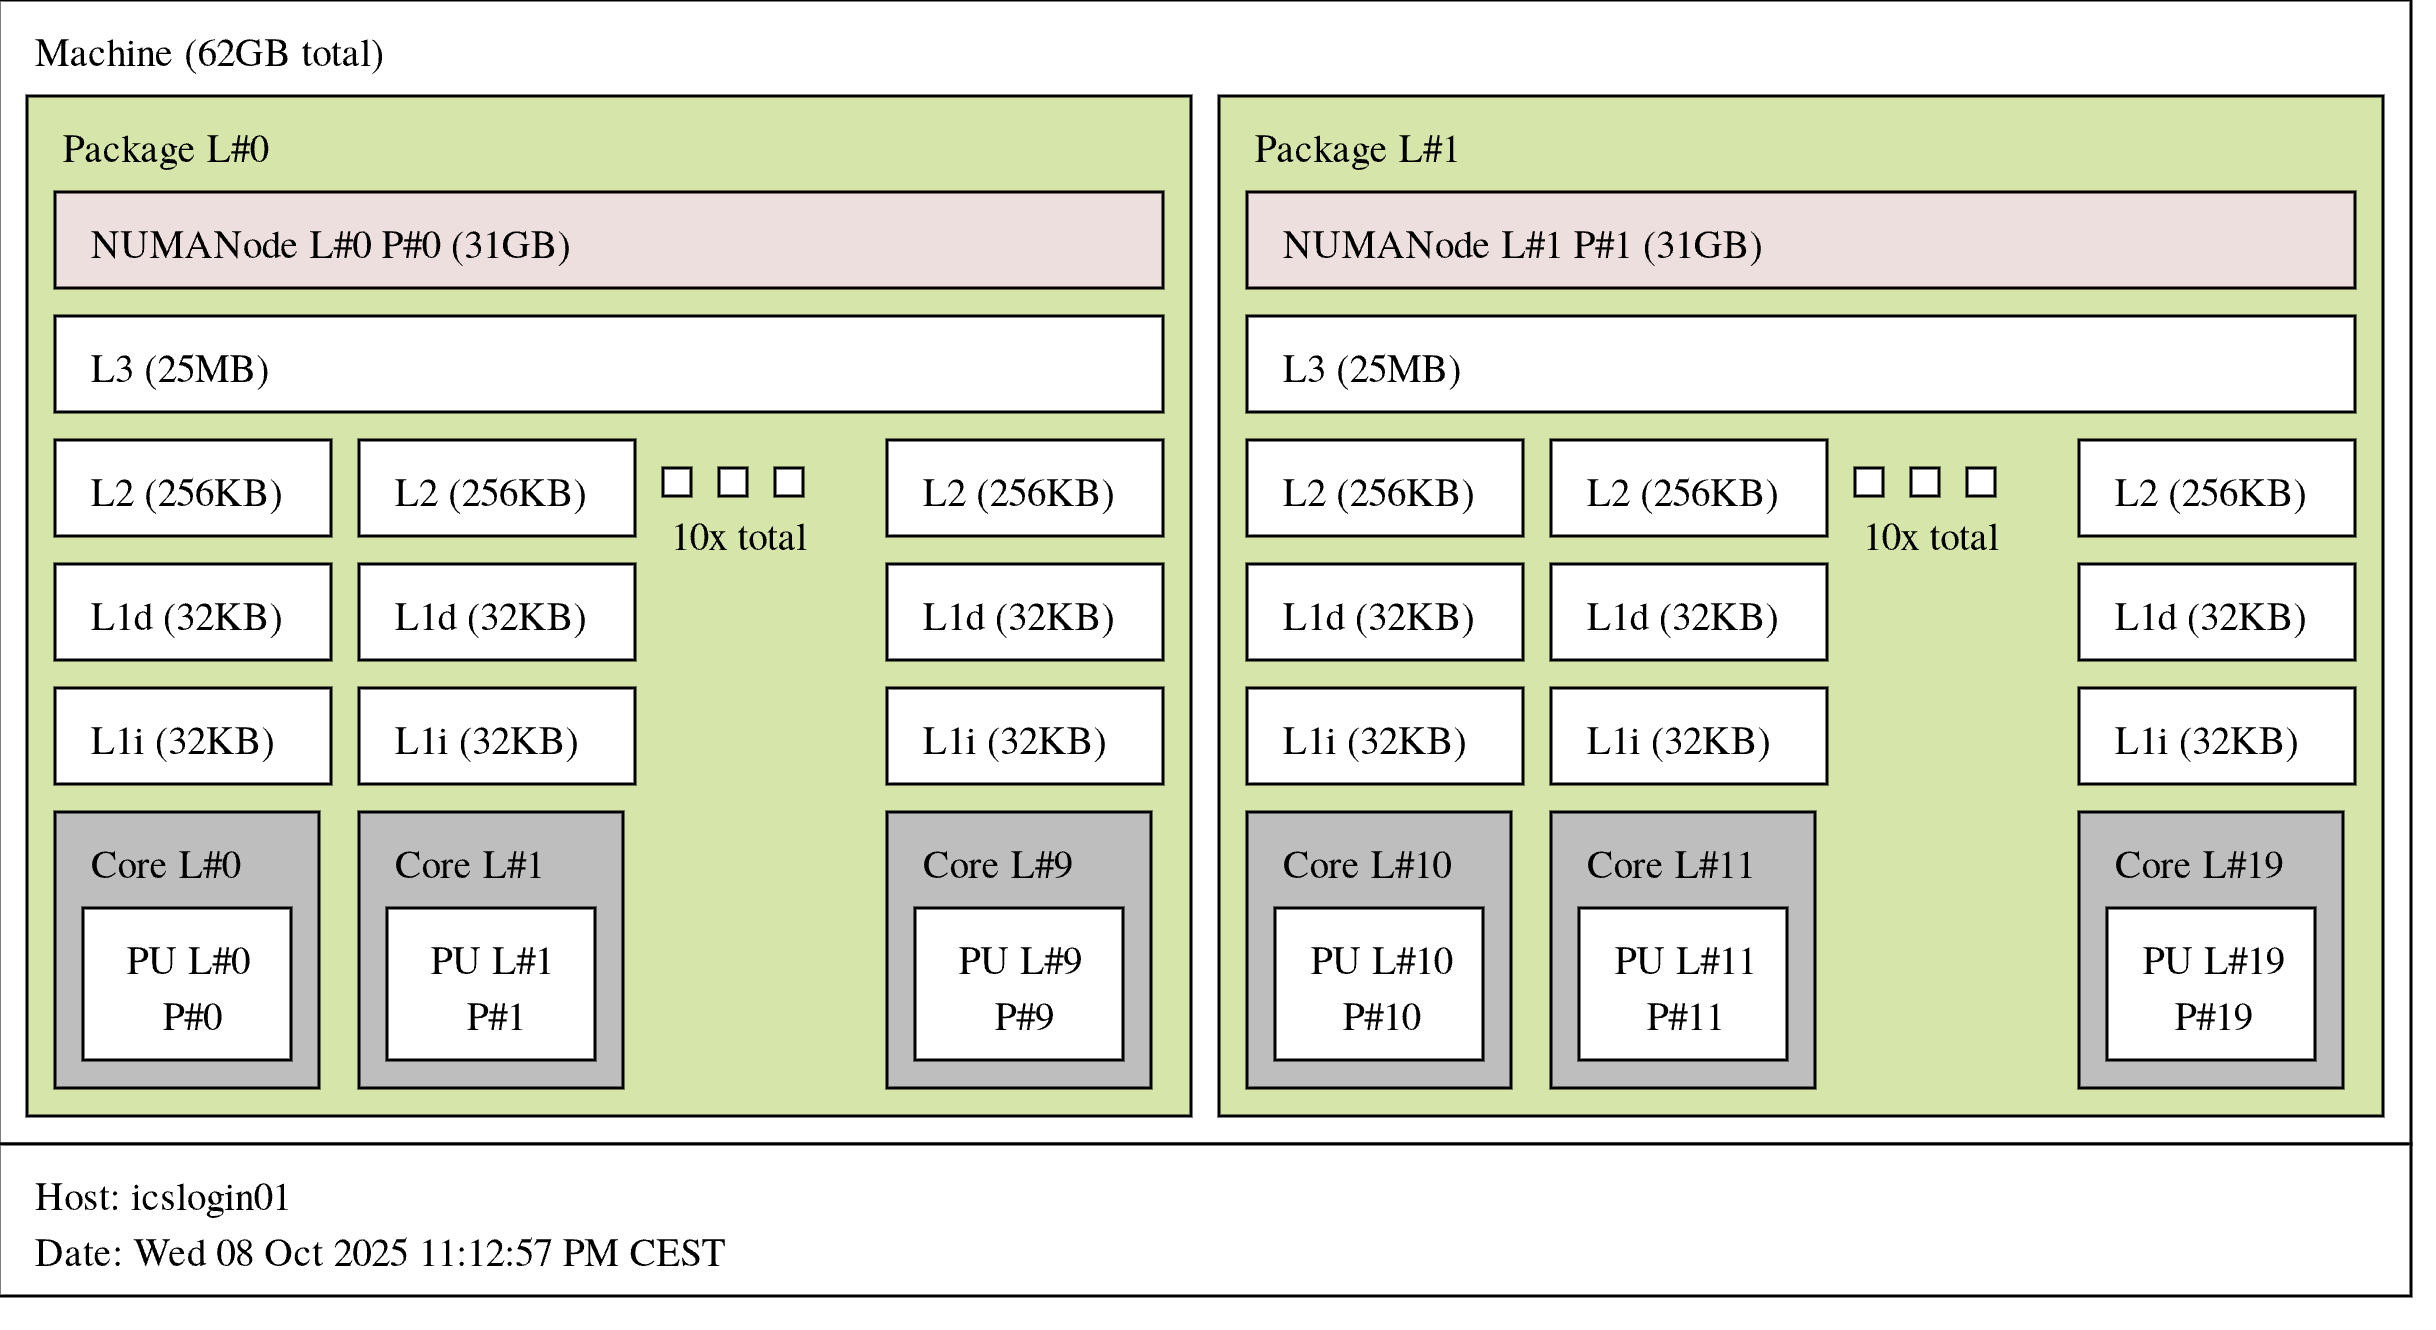
\includegraphics[width=0.9\textwidth]{../src/2-Performance-characteristics/02/XEON_E5-2650.png}
\caption{Graphical representation of Rosa node topology generated by command \texttt{hwloc-ls}.}
\label{fig:memory_topology}
\end{figure}


\subsection{Bandwidth: STREAM benchmark}
\label{subsec:stream}

The STREAM benchmark was executed on a single core of a Rosa consisting of four simple vector operations: Copy, Scale, Add, and Triad.

As required I runned the command:
\begin{verbatim}
    gcc -O3 -march=native -DSTREAM_TYPE=double -DSTREAM_ARRAY_SIZE=128000000 
        -DNTIMES=20 stream.c -o stream_c.exe
\end{verbatim}

So the array size is configured to 128,000,000 elements (~3GB) which significantly exceeds the L3 cache size (25MB), ensuring that the operations always "fall" out of the cache and therefore forcing the use main memory. This is done to \textbf{measure the bandwidth of main memory rather than cache performance.} Each kernel has been executed 20 times, and the best time (excluding the first iteration) I used to compute the reported bandwidth.

The complete output is available in the submission folder. The key results are shown below:

\lstinputlisting[
    caption={STREAM benchmark output on Rosa compute node (single-core)},
    captionpos=b,
    label={lst:stream-output},
]{../src/2-Performance-characteristics/03/slurm-52026.out}

The Copy operation shows substantially higher bandwidth (approximately 19GB/s) compared to the others.

The \textbf{Triad kernel bandwidth} of approximately 12.3 GB/s will be the average representative as memory bandwidth for a single core on Rosa compute nodes.

\subsection{Performance model: A simple roofline model}
\label{subsec:roofline}

Using the values obtained from the previous sections:
\begin{itemize}
    \item Peak performance per core: $P_{max} = 36.8$ GFlops/s (Section~\ref{subsec:peak_fp})
    \item Memory bandwidth per core: $b_{max} = 12.3$ GB/s (Section~\ref{subsec:stream})
\end{itemize}

The ridge point (performance transitions from memory-bound to compute-bound) occurs at:
\[
I_{ridge} = \frac{P_{max}}{b_{max}} = \frac{36.8}{12.3} \approx 2.99~\mathrm{Flops/Byte}
\]

\begin{figure}[h]
    \centering
    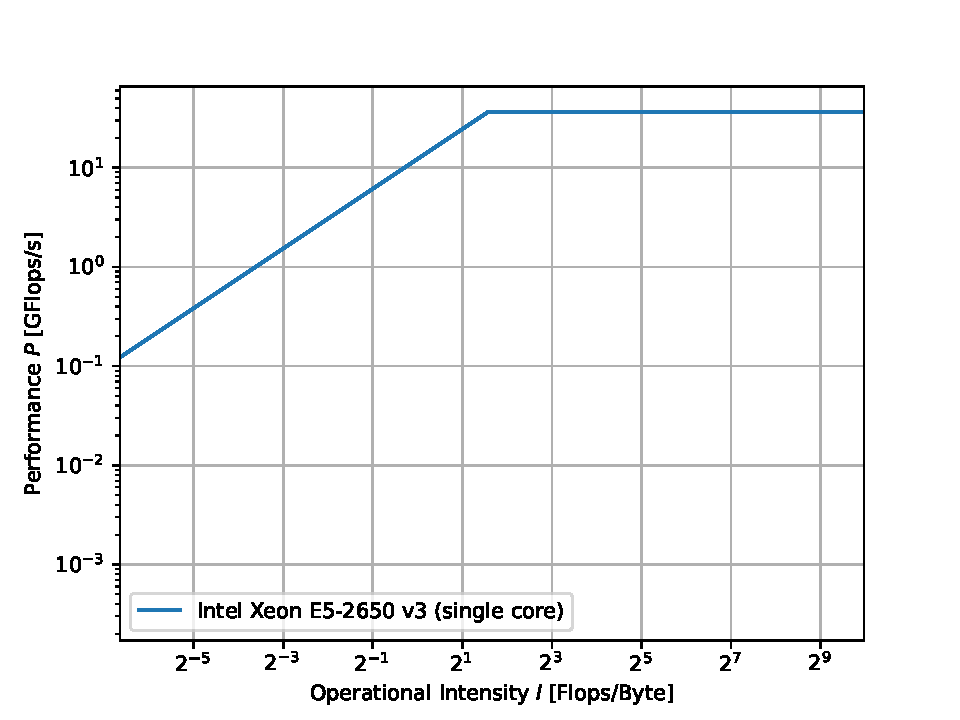
\includegraphics[width=0.9\textwidth]{../src/2-Performance-characteristics/04/roofline.pdf}
    \caption{Roofline model for Intel Xeon E5-2650 v3 (single core) on Rosa compute node.}
    \label{fig:roofline}
\end{figure}



\section{Optimize Square Matrix-Matrix Multiplication  \punkte{50}}

\subsection{Basic Blocked DGEMM}

I implemented the blocked \href{./../src/3-Optimize-Matrix-Matrix-Mult/dgemm-blocked.c}{DGEMM} has prescribed in the assignment and processed it on the cluster with different block sizes; the plots below \ref{fig:dgemm-performance} collect the timing traces.

\begin{figure}[h]
    \centering
    \begin{subfigure}[b]{0.48\textwidth}
        \centering
        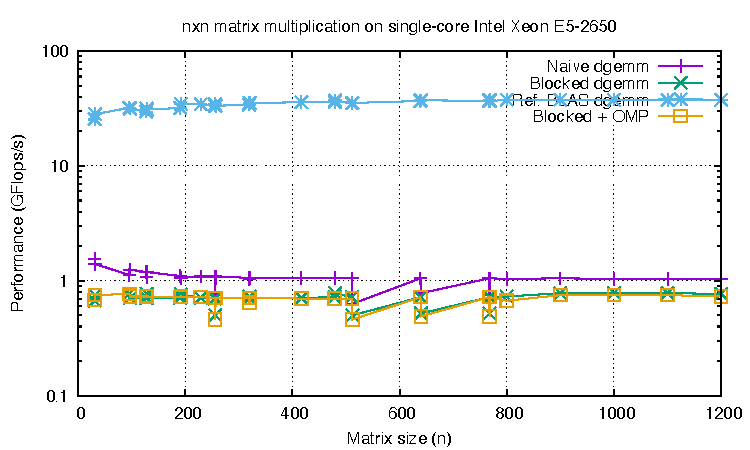
\includegraphics[width=\textwidth]{../src/3-Optimize-Matrix-Matrix-Mult/dgemm-blocked/timing-02.pdf}
        \caption{Block size = 2}
        \label{fig:timing-02}
    \end{subfigure}
    \hfill
    \begin{subfigure}[b]{0.48\textwidth}
        \centering
        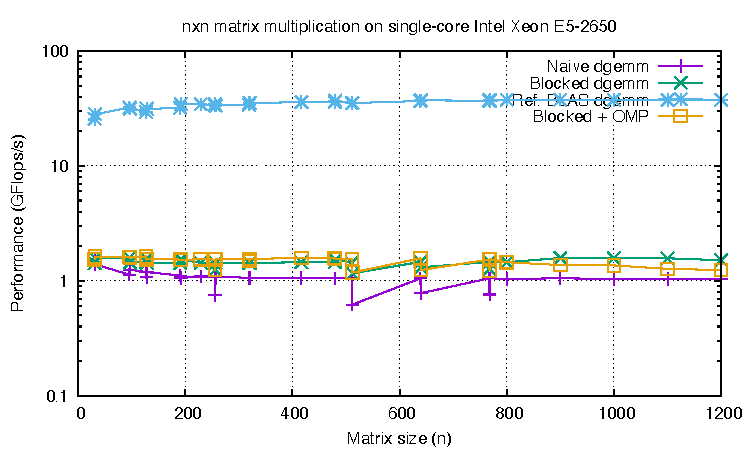
\includegraphics[width=\textwidth]{../src/3-Optimize-Matrix-Matrix-Mult/dgemm-blocked/timing-04.pdf}
        \caption{Block size = 4}
        \label{fig:timing-04}
    \end{subfigure}
    
    \vspace{1em}
    
    \begin{subfigure}[b]{0.48\textwidth}
        \centering
        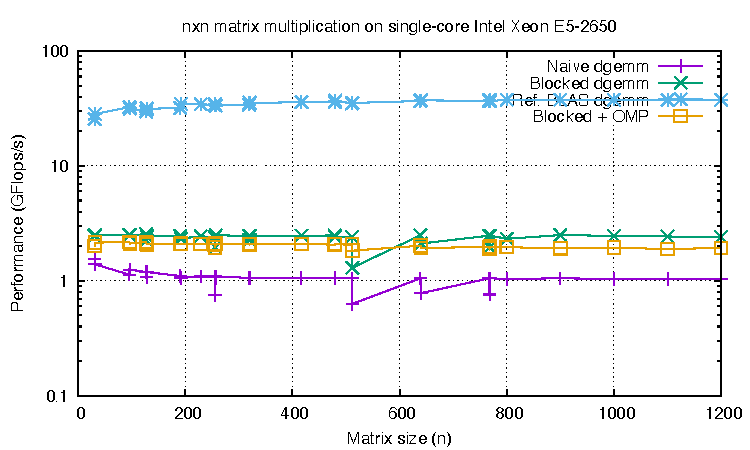
\includegraphics[width=\textwidth]{../src/3-Optimize-Matrix-Matrix-Mult/dgemm-blocked/timing-08.pdf}
        \caption{Block size = 8}
        \label{fig:timing-08}
    \end{subfigure}
    \hfill
    \begin{subfigure}[b]{0.48\textwidth}
        \centering
        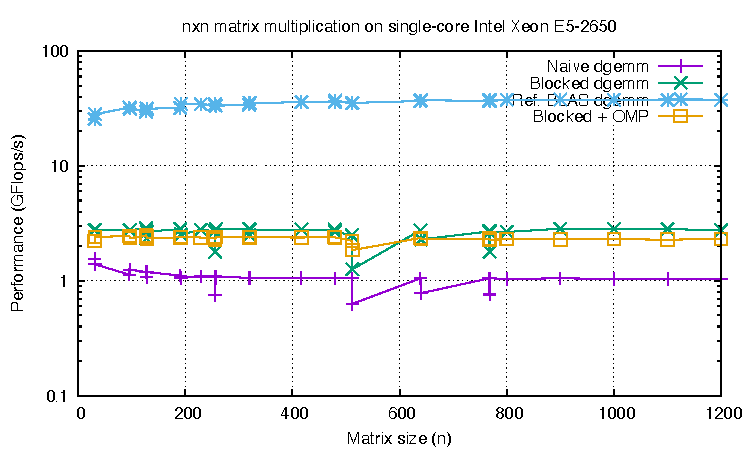
\includegraphics[width=\textwidth]{../src/3-Optimize-Matrix-Matrix-Mult/dgemm-blocked/timing-16.pdf}
        \caption{Block size = 16}
        \label{fig:timing-16}
    \end{subfigure}
    
    \vspace{1em}
    
    \begin{subfigure}[b]{0.48\textwidth}
        \centering
        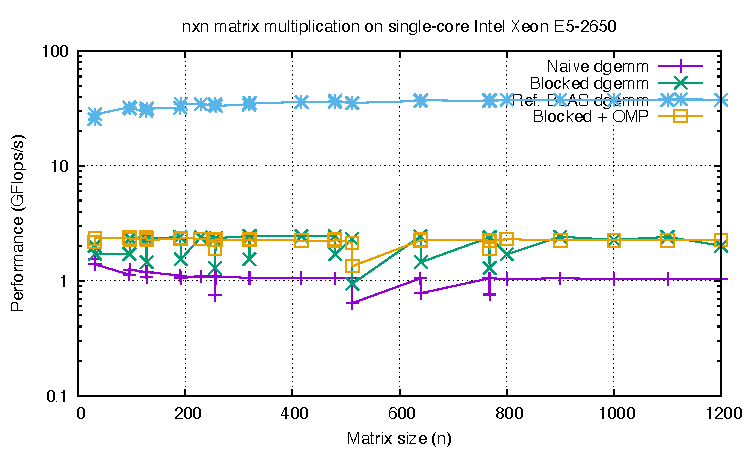
\includegraphics[width=\textwidth]{../src/3-Optimize-Matrix-Matrix-Mult/dgemm-blocked/timing-32.pdf}
        \caption{Block size = 32}
        \label{fig:timing-32}
    \end{subfigure}
    \hfill
    \begin{subfigure}[b]{0.48\textwidth}
        \centering
        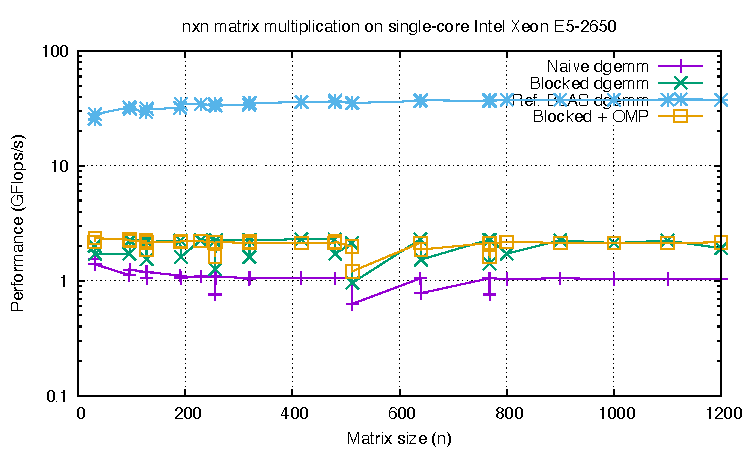
\includegraphics[width=\textwidth]{../src/3-Optimize-Matrix-Matrix-Mult/dgemm-blocked/timing-64.pdf}
        \caption{Block size = 64}
        \label{fig:timing-64}
    \end{subfigure}
    
    \caption{Performance comparison of different DGEMM implementations with diffenet block sizes}
    \label{fig:dgemm-performance}
\end{figure}

I summarized each result from the \texttt{.out} file in the \href{./../src/3-Optimize-Matrix-Matrix-Mult/basic-dgemm-blocked}{basic-dgemm-blocked folder} and reported them in the Table~\ref{tab:performance-summary}. This includes the averages and the quick binary-search that made block size 16 the best result so far at 7.08\% of peak. Of course a more refinded search could still find a better configuration.

\begin{table}[h]
\centering
\caption{Average Percentage of Peak Performance}
\label{tab:performance-summary}
\begin{tabular}{|l|c|c|c|}
\hline
\textbf{Implementation} & \textbf{Block Size} & \textbf{Avg. \% Peak} & \textbf{Notes} \\
\hline
\hline
Naive DGEMM & -- & 2.88\% & Independent of block size \\
\hline
BLAS DGEMM & -- & 93.77\% & Reference implementation \\
\hline
\hline
\multirow{6}{*}{Blocked DGEMM} 
& 2  & 1.91\% & \\
\cline{2-4}
& 4  & 3.97\% & \\
\cline{2-4}
& 8  & 6.41\% & \\
\cline{2-4}
& 16 & 7.08\% & Best blocked performance \\
\cline{2-4}
& 32 & 5.54\% & \\
\cline{2-4}
& 64 & 5.37\% & \\
\hline
\end{tabular}
\end{table}




\section{Quality of the Report  \punkte{15}}

\bibliographystyle{plain}
\bibliography{references}

\end{document}
